%%%%
% Project report based on the DAT620 template (ACM sigconf),
% edited by Leander Jehl and Hein Meling.
\documentclass[sigconf]{acmart}

%DON'T CHANGE THIS FILE
%This file sets several properties for the ACM template.
%It is not necessary to change this file.


% Copyright
\setcopyright{none}

% DOI
\acmDOI{}

% ISBN
\acmISBN{}

%Conference
\acmConference[Project in Computer Science (DAT620)]{}{IDE}{UiS}
\acmBooktitle{}
\copyrightyear{2018}

\newcommand{\supervisors}[1]{\thanks{Supervised by #1}}


%In the preamble file you can include packages and define macros.
% Packages and macros for the report.
% acmart already loads graphicx, xcolor, hyperref, amsmath and natbib.
\usepackage{booktabs}
\usepackage{tabularx}
\usepackage{listings}
\usepackage{enumitem}
\usepackage{tikz}
\usetikzlibrary{positioning,arrows.meta,fit}
\usepackage{colortbl}

\graphicspath{{figures/}}
\setlist[itemize]{topsep=0.2em, itemsep=0.15em, leftmargin=*}
\setlist[enumerate]{topsep=0.2em, itemsep=0.15em, leftmargin=*}
\setlength{\emergencystretch}{3em}

\newcommand{\code}[1]{\texttt{#1}}
\newcommand{\rowline}{\arrayrulecolor{black!25}\midrule\arrayrulecolor{black}}

\definecolor{codebg}{gray}{0.96}
\definecolor{codecomment}{rgb}{0.35,0.45,0.35}
\definecolor{codekw}{rgb}{0.10,0.25,0.55}
\lstset{
  language=Python,
  basicstyle=\ttfamily\scriptsize,
  backgroundcolor=\color{codebg},
  keywordstyle=\color{codekw}\bfseries,
  commentstyle=\color{codecomment}\itshape,
  stringstyle=\color{black!70},
  frame=single, rulecolor=\color{black!20},
  breaklines=true, columns=fullflexible,
  showstringspaces=false,
  xleftmargin=2pt, xrightmargin=2pt,
  aboveskip=0.5em, belowskip=0.3em
}


\begin{document}
\title{Rogaland Transit Medallion}
\subtitle{How punctual are the buses in Rogaland?\\DAT535 Data Engineering, Group 5}

%TODO: fill in the emails
\author{Tommaso Facchin}
\affiliation{University of Stavanger, Norway}
\email{tofac4317@stud.uis.no}

\author{Oliwier Trawinski}
\affiliation{University of Stavanger, Norway}
\email{TODO@stud.uis.no}

%TODO: add the name of one or more supervisors
\supervisors{TODO}

\begin{abstract}
\noindent
Entur's live API for Kolumbus buses in Rogaland keeps no history, so we built it ourselves.
We save the feed every 5 minutes in Bronze, turn about 3.4 million repeated stop rows per day
into 153{,}000 stop calls in Silver, and group them into three punctuality tables in Gold. It
runs on two OpenStack VMs with PySpark and GitHub Actions. Over 27 days (27 October to
22 November 2026), 55\% of stops are on time, 15:00 on weekdays is the worst hour (33\%), and
X39 is the worst line (14\%).

\end{abstract}

\keywords{Data engineering, medallion architecture, PySpark, public transport}

\maketitle

\section{Scope}
We want to find out which Kolumbus lines, stops and hours are least punctual. A planner at
Kolumbus or in the county could use this to decide which timetables to fix first. We picked
this data because we use these buses ourselves, and because it forced real decisions: the API
only shows the current state, and every answer repeats all running trips.

Some things are not part of the project:
\begin{itemize}
  \item \textbf{Live (streaming) results.} A report once a night is enough for this question.
  \item \textbf{Trips that are not in the live feed at all.} We can only measure trips that
        Entur sends. Finding missing trips would need the full timetable (GTFS).
  \item \textbf{Passenger numbers and a finished dashboard.} Gold is read with Spark SQL and
        charts (Section~\ref{sec:results}).
\end{itemize}

We wrote the layers as Python modules with one entry point (\code{jobs/run\_pipeline.py})
instead of notebooks, because modules are easier to schedule and to test.


\section{Medallion architecture}
Each layer has its own folder on the prod VM and only reads the layer below it
(Figure~\ref{fig:arch}, Table~\ref{tab:layers}). Cron saves a Bronze snapshot every 5 minutes.
Every night a GitHub Actions run does four steps in order: it saves a fresh copy of the line
list in Bronze, builds Silver for the day before, rebuilds the line names table from the saved
lists, and builds Gold.

\begin{figure*}[t]
\centering
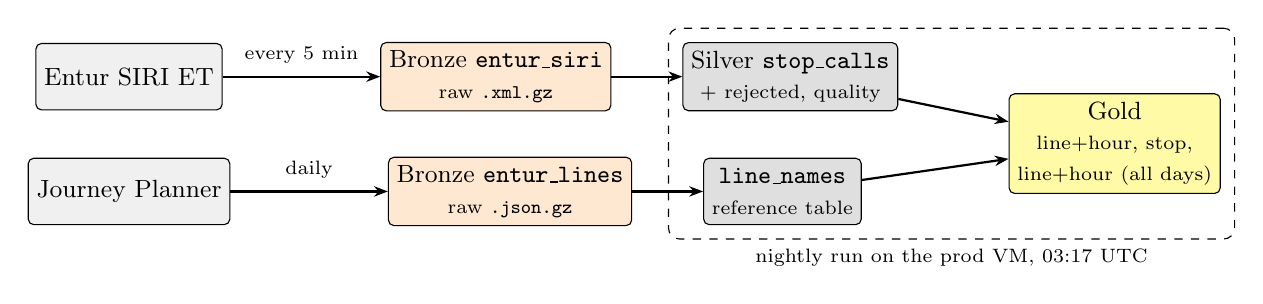
\begin{tikzpicture}[
  font=\small,
  box/.style={draw, rounded corners=2pt, align=center, minimum height=2.4em, inner sep=3pt},
  src/.style={box, fill=gray!12},
  bro/.style={box, fill=orange!18},
  sil/.style={box, fill=gray!25},
  gol/.style={box, fill=yellow!35},
  arr/.style={-{Stealth[length=5pt]}, thick},
  lab/.style={font=\scriptsize, midway, above=1pt}
]
\node[src] (siri) {Entur SIRI ET};
\node[src, below=0.6cm of siri] (jp) {Journey Planner};
\node[bro, right=2.0cm of siri] (b1) {Bronze \code{entur\_siri}\\\scriptsize raw \code{.xml.gz}};
\node[bro, right=2.0cm of jp] (b2) {Bronze \code{entur\_lines}\\\scriptsize raw \code{.json.gz}};
\node[sil, right=0.9cm of b1] (s) {Silver \code{stop\_calls}\\\scriptsize + rejected, quality};
\node[sil, right=0.9cm of b2] (r) {\code{line\_names}\\\scriptsize reference table};
\node[gol, right=1.4cm of s, yshift=-0.85cm] (g) {Gold\\\scriptsize line+hour, stop,\\\scriptsize line+hour (all days)};
\draw[arr] (siri) -- node[lab]{every 5 min} (b1);
\draw[arr] (jp) -- node[lab]{daily} (b2);
\draw[arr] (b1) -- (s);
\draw[arr] (b2) -- (r);
\draw[arr] (s) -- (g);
\draw[arr] (r) -- (g);
\node[draw, dashed, rounded corners, inner sep=5pt, fit=(s)(r)(g),
      label={[font=\scriptsize]below:nightly run on the prod VM, 03:17 UTC}] {};
\end{tikzpicture}
\caption{The pipeline. Both outside sources are saved raw in Bronze before anything else
reads them. All data lives on the prod VM in \code{/data/entur}.}
\label{fig:arch}
\end{figure*}

\begin{table*}[t]
\caption{What each layer holds and how we keep the layers apart.}
\label{tab:layers}
\centering\small
\renewcommand{\arraystretch}{1.25}
\begin{tabularx}{\textwidth}{@{}l>{\raggedright}X>{\raggedright\arraybackslash}p{6.2cm}@{}}
\toprule
Layer & What is stored & Rules \\
\midrule
Bronze & Every API answer as received (SIRI every 5 min, line list daily), gzipped, plus one metadata line per run &
  Never changed or overwritten. Failed and broken answers are kept and marked. \\ \rowline
Silver & One row per stop of a trip and service day; rejected rows; a quality table. The line names table (\code{reference/}) is built the same way &
  Built only from Bronze. Times in UTC, duplicates removed, problems flagged. A rerun replaces only the days it builds. \\ \rowline
Gold & Three small tables: punctuality per line and hour, per stop (per service day), and per line and hour over all days &
  Built only from Silver. Written only if Silver looks complete. The all-days table is rebuilt from all of Silver on every run. \\
\bottomrule
\end{tabularx}
\end{table*}

Table~\ref{tab:decisions} lists the main decisions. The full log with dates and owners is
\code{docs/decisions.md} in the repository~\cite{repo}.

\begin{table*}[t]
\caption{Main decisions.}
\label{tab:decisions}
\centering\small
\renewcommand{\arraystretch}{1.3}
\begin{tabularx}{\textwidth}{@{}>{\raggedright}p{4.3cm}>{\raggedright}X>{\raggedright\arraybackslash}p{4.3cm}@{}}
\toprule
Problem & What we chose & Evidence \\
\midrule
The API keeps no history & Start collecting before writing any Silver code & Collection runs since 27 Oct \\ \rowline
Finished trips leave the feed after a few minutes & Poll every 5 minutes instead of 15 & Trips stay 4--11 min after the last stop \\ \rowline
2.6\,GB of raw data a day & Store Bronze gzipped & About 15 times smaller \\ \rowline
GitHub schedules start late & Cron on the VM for Bronze & 7{,}778 runs, no gap over 10 min \\ \rowline
The feed has no line numbers & Save Entur's line list in Bronze every day & 320 lines, all Silver lines named \\ \rowline
Shares cannot be added over days & Gold stores counts & Exact share for any period \\ \rowline
A day can be incomplete & Write Gold only if Silver looks complete & All 27 days passed \\ \rowline
200 shuffle tasks for 150k rows & 8 shuffle partitions & Gold 28\,s $\rightarrow$ 17\,s \\ \rowline
Silver read 3 Bronze days per day & Read only the hours it needs & 864 $\rightarrow$ 372 files, 308\,s $\rightarrow$ 141\,s \\ \rowline
Spark's XML reader dropped the \code{+01:00} offset & Parse with Python's ElementTree inside Spark, one task per file & No shifted times; no more out-of-memory \\ \rowline
Each stop is in about 22 snapshots & Window: recorded first, newest snapshot, then \code{run\_id} & 3.4\,M $\rightarrow$ 153k rows, same result on every rerun \\ \rowline
A bad row could hide a delay or break Gold & Reject only rows that can never give a delay, flag the rest & 0 rejected rows in 27 days \\ \rowline
Silver can be wrong without an error & Quality table with 23 metrics per run & Every day checked in Figure~\ref{fig:quality} \\ \rowline
The repository is public & Tests on GitHub's machines, never on our VMs & PR code never runs on our servers \\ \rowline
Manual deploys drift apart & Deploy on merge: \code{dev} to dev VM, \code{main} to prod & Both VMs run reviewed code \\ \rowline
Silver and Gold need logs and a status & Nightly run in GitHub Actions at 03:17 UTC & Red run below 270 of 288 snapshots \\
\bottomrule
\end{tabularx}
\end{table*}


\section{The data}
\label{sec:data}
We use Entur's real-time API for the SIRI Estimated Timetable~\cite{entur}. It is free and
open (NLOD licence~\cite{nlod}) and needs no key. Each call returns one XML file of about 9\,MB
with all Kolumbus trips running at that moment. For every trip it lists the stops already
passed, with real times, and the stops ahead, with predicted times. To get only Kolumbus we
use the parameter \code{datasetId=KOL}; the parameter in our first plan
(\code{datasource=KOL}) did not filter anything.

Since the API only shows the present, every day without collection is lost for good. So we
started Bronze on 26 October, before any Silver code existed. While it was running, we studied
the raw files and found what Silver had to handle: times with a local offset (\code{+01:00})
just after a clock change, each stop repeated in about 22 snapshots, no line numbers, a missing
\code{Cancellation} field, broken stop names (\code{Ã} instead of \code{ø}) and several route
variants per line.

At 288 snapshots a day this is about 5.3 million stop rows and 2.6\,GB before compression,
and the archive grows every day. The work splits naturally by file, which is why we use Spark,
even though the Gold tables are small.


\section{Platform on OpenStack}
\label{sec:platform}
\begin{itemize}
  \item \textbf{Two VMs.} \code{dat535-dev} is for trying changes on a small copy of the data,
        \code{dat535-prod} for collection and the nightly run. Both are \code{m1.large}
        (4 cores, 8\,GB RAM) with Java 17 and PySpark 4.1.3, and run the same code with their
        own config file.
  \item \textbf{One floating IP.} Our quota has only one, so prod has it and we reach dev
        through prod with SSH \code{ProxyJump}.
  \item \textbf{Data on its own volume.} All data is on a separate 200\,GB volume on
        \code{/data}, so it survives a rebuilt VM.
  \item \textbf{Spark in local mode on one VM.} A weekday of Bronze is only 124\,MB compressed,
        and a cluster over our two VMs would mix dev and prod. Every step works per file or per
        day, so the same code could run on a real cluster if the data grew.
  \item \textbf{Self-hosted GitHub runners.} GitHub's machines cannot reach our VMs, so each
        VM runs its own runner. The runners only run merged code (deploy and the nightly run),
        never code from a pull request (Section~\ref{sec:lifecycle}).
  \end{itemize}


\section{Bronze}
\label{sec:bronze}
\subsection*{How often to poll}

Our first plan was to poll every 15 minutes. Before we started, we tested how long a finished
trip stays in the feed: on 26 October we saved 32 snapshots, 5 minutes apart, and compared the
last snapshot of each trip with the time of its last stop (\code{scripts/retention\_check.py}).
Of 771 trips that left the feed, all stayed between 4 and 11 minutes after the last stop
(median 8), and none stayed 15. So 15 minutes would have been too slow: for most trips we would
never see the real time at the last stops.

With 5 minutes, almost every trip is seen after it has finished. A trip that leaves after only
4 minutes can still fall between two polls, and then its last stops keep the predicted time
instead of the real one. We count these stops in every Silver run: 0.2--1.8\% a day. Leaving
them out changes the on-time share by only 0.05 points, so we keep them. Polling more often
would save these few stops but multiply storage and API calls.

\subsection*{How the raw data is kept}

\begin{itemize}
  \item Every answer is saved exactly as received, gzipped (about 15 times smaller, and Spark
        reads it directly), in folders by UTC date and hour.
  \item Every run, also a failed one, adds one line to a metadata file: time, HTTP status, size,
        checksum and error. Broken XML is saved too and marked as broken.
  \item A file is never overwritten, and every Silver row keeps the id of its Bronze file, so
        any number in Gold can be traced back to one raw answer.
\end{itemize}

Bronze runs from cron on the prod VM, not from a GitHub schedule. When we tried both, every
snapshot was fetched twice, and GitHub's scheduled runs started minutes late, which is enough
for a trip to leave the feed. From 27 October to 22 November there were 7{,}778 runs, one
failed (a DNS error on 29 October), and there was no gap longer than 10 minutes.

\subsection*{Line names come from Bronze too}

The feed only has line ids like \code{KOL:Line:8\_2043}. Entur's Journey Planner~\cite{jp}
knows the public number (here X39). Our first version called this API and wrote the answer
directly into a table, so the raw answer was never kept. We got this feedback at the
presentation and changed it:
\begin{itemize}
  \item The step \code{bronze-lines} saves the full Kolumbus line list (320 lines) once a day in
        its own Bronze folder, raw, with a metadata line, the same way as the SIRI data.
  \item The step \code{lines} reads all saved lists with Spark and keeps the newest name for
        each line id. A line that stops running keeps its last name.
  \item If the API is down, we only get a warning and Gold uses the lists already saved.
\end{itemize}

\begin{lstlisting}
w = Window.partitionBy("line") \
          .orderBy(F.col("fetched_at").desc())
names = lines.withColumn("_rn", F.row_number().over(w)) \
             .filter("_rn = 1").drop("_rn")
\end{lstlisting}


\section{Silver}
\label{sec:silver}
\subsection*{Grain and key}

One Silver row is one stop of one trip on one service date, with the key
\code{journey\_id + service\_date + stop\_order}. That is the smallest unit where punctuality
makes sense, and it keeps Silver useful for other questions than ours. \code{service\_date}
comes from \code{DataFrameRef} in the feed, not from the clock, so a trip at 00:30 belongs to
the right operating day. Silver also computes the arrival and departure delay in seconds
(actual or expected minus aimed) and keeps \code{snapshot\_time}, \code{run\_id} and
\code{call\_status} (recorded or estimated).

\subsection*{Parsing}

We tried Spark's XML reader first. It dropped the \code{+01:00} from the timestamps, which
would have shifted every delay by an hour without any error, and it gave recorded and
estimated stops different structures. So we parse each file with Python's ElementTree inside
Spark tasks and convert all times to UTC:

\begin{lstlisting}
# 20:00 the day before to 02:59 the day after
paths = list_bronze_files(root, start, end)
# one task per file, so a task only holds one snapshot in memory
results = sc.parallelize(paths, len(paths)).map(read_file) \
            .persist(StorageLevel.MEMORY_AND_DISK)
\end{lstlisting}

One task per file comes from our first prod run, which ran out of memory: Spark had put 288
files into 4 big tasks. Bronze folders are UTC days, while a night bus of day $D$ can show up
in the files of the next day, so Silver reads from 20:00 the evening before to 02:59 the
morning after, and only writes day $D$ (Section~\ref{sec:perf}).

\subsection*{Reject or flag}

A rejected row is gone for the analysis, while a flagged row can still be used or left out
later. So we only reject rows that can never give a delay and flag the rest
(Table~\ref{tab:rules}). Rejected rows are saved in \code{silver/rejected\_calls} with the code
of the first rule they fail. The rules run before deduplication, so a broken row can never be
the copy that is kept. In 27 days no row was rejected.

\begin{table}[htb]
\caption{Silver rules. Cancelled trips stay in Silver so Gold can count cancellations.}
\label{tab:rules}
\centering\small
\renewcommand{\arraystretch}{1.2}
\begin{tabularx}{\linewidth}{@{}ll>{\raggedright\arraybackslash}X@{}}
\toprule
& Rule & Why \\
\midrule
Reject & \code{MISSING\_KEY} & no journey, service date or stop order, so no deduplication \\
Reject & \code{MISSING\_LINE\_OR\_STOP} & cannot be grouped in Gold \\
Reject & \code{MISSING\_AIMED\_TIME} & no aimed time, so no delay \\ \rowline
Flag & \code{is\_missing\_actual} & no actual or expected time \\
Flag & \code{is\_delay\_outlier} & delay below $-10$\,min or above 3\,h \\
Flag & \code{is\_bad\_stop\_name} & name contains \code{Ã} (UTF-8 read as Latin-1) \\
Flag & \code{exclude\_from\_punctuality} & cancelled, outlier or no actual time \\
\bottomrule
\end{tabularx}
\end{table}

The outlier limits were a guess at first. We checked them on 11 days of prod data: 99.8\% of
stops are between $-5$ and $+60$ minutes, with a median of $+2.2$. The 702 stops below
$-10$ minutes were mostly times from the day before, and the 17 above 3 hours came from two
trips shifted by 4 to 11 hours on every stop. These are feed errors, so we kept the limits.

\subsection*{Removing duplicates}

Every stop is repeated in about 22 snapshots. On 2 November the snapshots had 3{,}401{,}155
stop rows, which became 153{,}568 stops. \code{dropDuplicates} would keep a random copy, but
we want the best one, so we use a window:

\begin{lstlisting}
w = Window.partitionBy("journey_id", "service_date",
                       "stop_order").orderBy(
    # real time before prediction
    (F.col("call_status") == "recorded").desc(),
    # then the newest snapshot
    F.col("snapshot_time").desc(),
    # same snapshot twice: stable choice
    F.col("run_id").desc())
df.withColumn("_rn", F.row_number().over(w)) \
  .filter("_rn = 1").drop("_rn")
\end{lstlisting}

We added \code{run\_id} after the double fetch on 27 October: two copies of the same snapshot
had the same \code{snapshot\_time}, Spark picked one at random, and two reruns of the same day
did not give the same result.

\subsection*{Quality table and reruns}

Every run appends its numbers to \code{silver/quality}, one row per metric (23 per run): rows
read, unparseable rows, rejected rows per reason, nulls, each flag, duplicates before and
after deduplication, a schema check, and files read and skipped. With one row per metric we can
add metrics without changing the table. Figure~\ref{fig:funnel} follows one day through
Silver, and Figure~\ref{fig:quality} shows the Silver rows and flags for every service day.

\begin{figure}[!htbp]
\centering
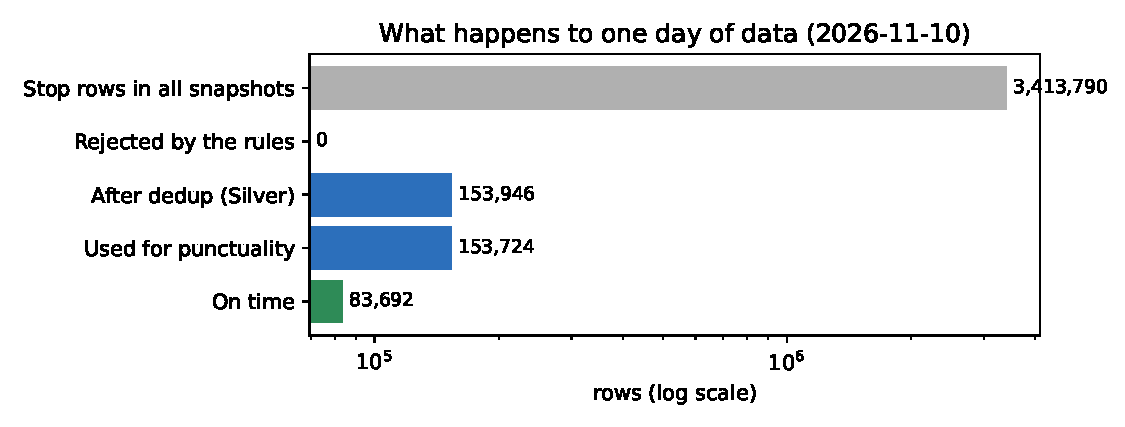
\includegraphics[width=0.85\linewidth]{3_silver_funnel.pdf}
\caption{One day through Silver, from the rows read to the rows written.}
\label{fig:funnel}
\end{figure}

\begin{figure*}[t]
\centering
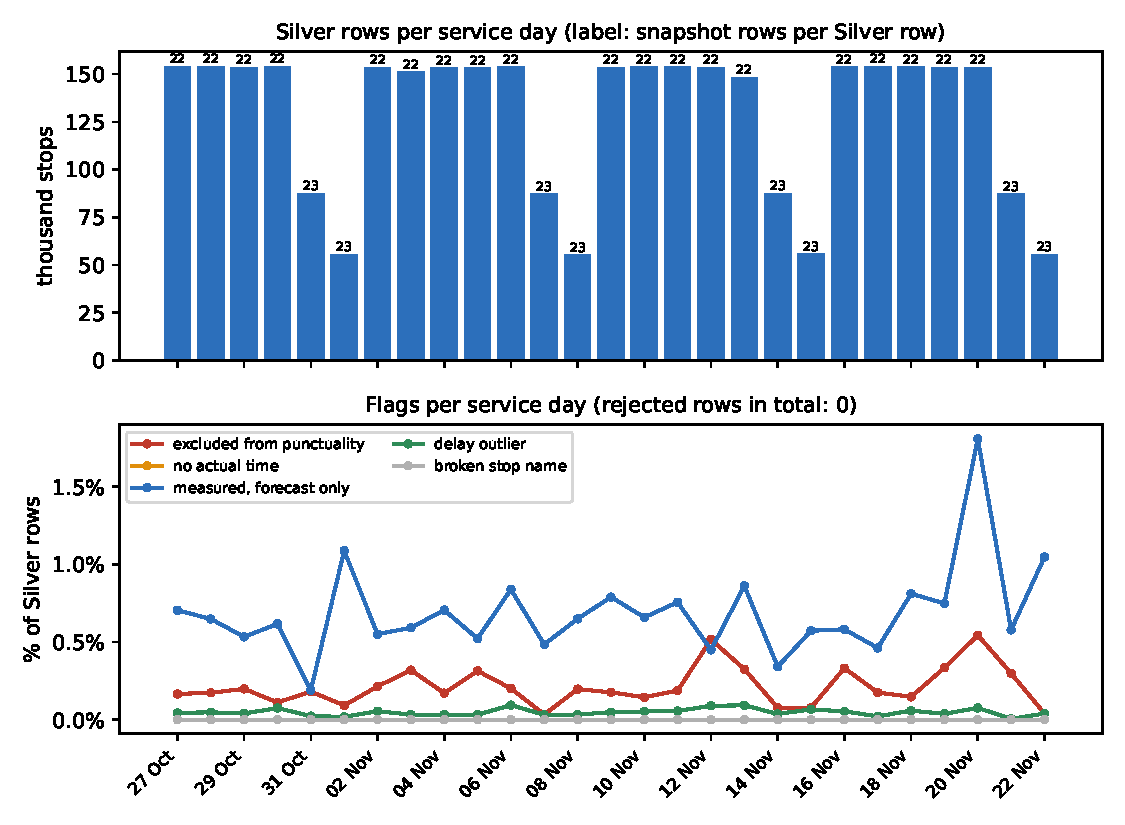
\includegraphics[width=0.85\textwidth]{7_quality_per_day.pdf}
\caption{Silver rows and flags per service day, from the quality table.}
\label{fig:quality}
\end{figure*}

A Bronze file that cannot be read is skipped and counted. If more than 5\% of the files fail,
Silver stops before writing anything: at that point a bug in our code is more likely than bad
data, and we do not want a good day replaced by a partial one. Silver is written as Parquet
partitioned by \code{service\_date} with dynamic partition overwrite, so a rerun only replaces
the days it builds.


\section{Gold}
\label{sec:gold}
Silver keeps about 150k stop rows a day, useful for many questions. Gold answers only ours, in
two small tables per service day (punctuality per line and hour, and per stop) and one table
per line and hour over the whole period.

How we count:
\begin{itemize}
  \item \textbf{On time} means from 1 minute early to 3 minutes late, based on the departure
        time (the arrival time at the last stop).
  \item \textbf{Cancelled trips} have no delay. They are left out of the on-time share, but
        counted for the cancellation rate.
  \item \textbf{The hour} is in Norwegian time. Silver keeps UTC, so Gold converts before
        grouping; otherwise the 8 o'clock rush would show up as 7.
  \item \textbf{Counts, not only percentages.} Each row stores how many stops were measured, on
        time, late and early. A percentage cannot be averaged over days, but counts can be
        added, so any period gives the exact share.
  \item \textbf{One table over all days.} Counts can be added over days, but the 90th
        percentile of the delay cannot: it needs all the rows. So Gold also keeps
        \code{punctuality\_by\_line\_hour\_all}, one row per line and hour over every day in
        Silver, with the number of days. It is rebuilt from all of Silver on every run.
\end{itemize}

Gold is only written when Silver looks complete. Before writing, it checks two things:
\begin{enumerate}[topsep=0.2em, itemsep=0.25em]
  \item \textbf{Is the day complete?} Every day needs at least 20{,}000 Silver rows (even a
        Sunday has about 55k). This catches missing data.
  \item \textbf{Is every stop counted exactly once?} The calls in each daily Gold table must add up
        to the Silver rows. This catches bugs in Gold, for example a line listed twice in the
        names table.
\end{enumerate}

\begin{lstlisting}
problems = [f"{d}: only {n} rows"
            for d, n in day_counts if n < 20_000]
if line_hour_calls != silver_rows \
        or stop_calls != silver_rows:
    problems.append("counts do not match")
if not problems:
    line_hour.repartition("service_date") \
        .write.mode("overwrite") \
        .partitionBy("service_date").parquet(...)
\end{lstlisting}

If a check fails, nothing is written, the old Gold stays, and the run is marked as failed in a
status file that also tells users when Gold was last updated. All 27 days passed. We read Gold
with Spark SQL, for example the least punctual lines:

\begin{lstlisting}[language=SQL]
SELECT line,
       sum(on_time_calls) / sum(measured_calls) AS on_time_share
FROM line_hour_all
GROUP BY line ORDER BY on_time_share LIMIT 10
\end{lstlisting}


\section{Testing, deployment and the nightly run}
\label{sec:lifecycle}
We work on feature branches, open a pull request to \code{dev}, and later merge \code{dev}
into \code{main}.

\textbf{Tests run on GitHub's machines, not on ours.} \code{tests.yml} runs ruff and pytest
for every push and pull request. The repository is public, so anyone can open a pull request,
and we did not want that code to run on our VMs. The tests use a small local Spark session,
so they need no data. On 23 November \code{ubuntu-latest} changed its default Java and Spark
could no longer write Parquet, so the workflow now pins Java 17, the same as on the VMs.

\textbf{Deploy on merge.} The self-hosted runners only run code that is already merged.
\code{deploy.yml} updates the dev VM on a merge to \code{dev} and the prod VM on a merge to
\code{main} (\code{git pull} and \code{pip install}), so the VMs never run code nobody reviewed.

\textbf{The nightly run.} \code{pipeline.yml} runs at 03:17 UTC on the prod runner, or by hand
for any day on dev or prod. Bronze stays on cron because it needs exact timing, while Silver
and Gold can start a bit late, and in Actions we get logs, history and a red or green status
for free. The first scheduled runs started up to 7.5 hours late; moving from 04:00 to 03:17
helped, because GitHub delays full-hour schedules the most.

\textbf{The run page tells us if the day is good.} At the end the workflow writes a summary
(Bronze runs, Silver rows, Gold status), also after a failure. On prod the run also turns red
with fewer than 270 of 288 valid snapshots: the 20{,}000-row check in Gold alone would let a
half day through.

% Results figure, placed here so the float lands before the Results section.
\begin{figure*}[t]
\centering
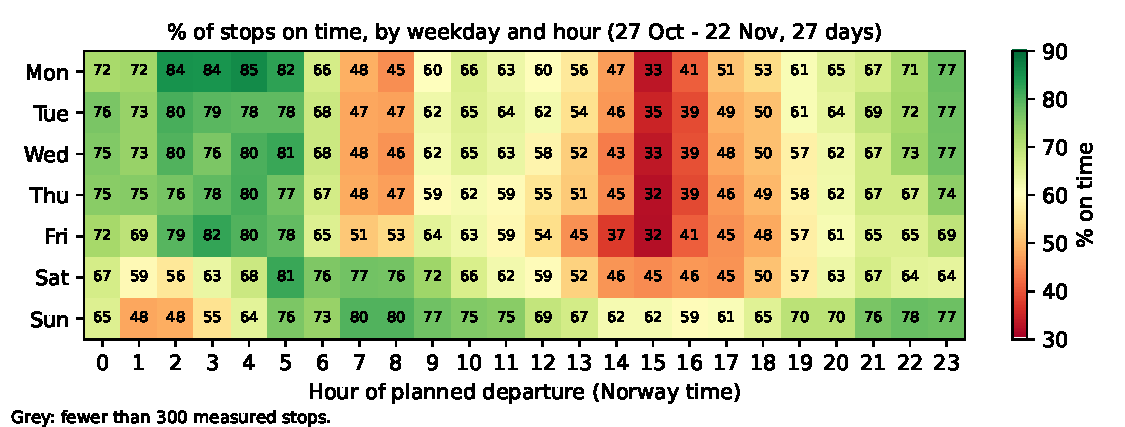
\includegraphics[width=0.85\textwidth]{1_heatmap_weekday_hour.pdf}
\caption{On-time share by weekday and hour of planned departure (Norwegian time).}
\label{fig:heatmap}
\end{figure*}


\section{Performance}
\label{sec:perf}
We changed Spark settings only after measuring. Each test ran one day of data on prod, and we
read the time of each stage from the Spark event logs~\cite{spark} (Figure~\ref{fig:perf}).
The panels use two versions of Silver: the \emph{old} one, which read three full Bronze days,
and the \emph{new} one with the read window described below. Panel (a) is the old version on
4~November data. Panel (c) compares the old and the new version on the same day, 6~November.

\begin{figure*}[t]
\centering
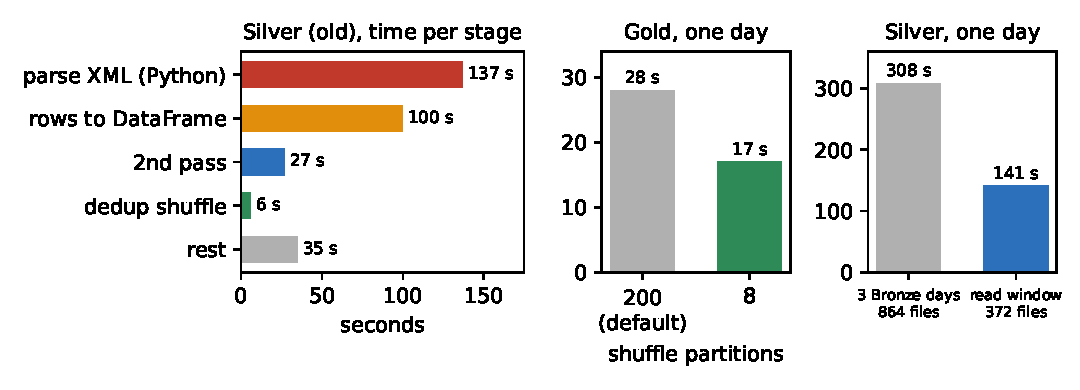
\includegraphics[width=0.7\textwidth]{5_performance.pdf}
\caption{(a) Old Silver (three Bronze days) on 4 November data: time per stage.
(b) Gold for one day with 200 and 8 shuffle partitions.
(c) Old and new Silver on the same day, 6 November: total time.}
\label{fig:perf}
\end{figure*}

\begin{itemize}
  \item \textbf{Gold: 8 shuffle partitions instead of 200.} Gold groups only about 150k rows a
        day, so 200 tasks were mostly overhead. With 8, Gold went from 28\,s to 17\,s.
  \item \textbf{Silver: Spark settings did not help.} The shuffle for removing duplicates takes
        only a few seconds. Most of the time is Python reading the XML files, and each Bronze
        day read costs about 100\,s. So the fix was to read fewer files.
  \item \textbf{Silver: read only the hours it needs.} A night bus that belongs to day $D$ can
        appear in the files of the next UTC day, so the first version read three full Bronze
        days (864 files) to build one day. We checked all 27 days: the stops of day $D$ appear
        from about 23:20 UTC the evening before until at most 01:15 the morning after. With
        2 hours of margin, Silver now reads from 20:00 the evening before to 02:59 the morning
        after (372 files). This cut the run from 308\,s to 141\,s, with exactly the same rows.
        It also makes reruns give the same result, because the old version read up to the
        moment the run started.
  \item \textbf{One Parquet file per day.} Silver and Gold are written with
        \code{repartition("service\_date")}, so each day is one file instead of one per task,
        and later reads open fewer small files. The Silver quality metrics are now computed in
        one aggregation instead of several separate counts.
\end{itemize}

The files between 20:00 and 03:00 UTC are still read by two nightly runs. Saving each parsed
Bronze file once, split by service day, would remove that too; we leave it as future work.


\section{Results}
\label{sec:results}
Over 27 days Silver has 3{,}485{,}540 stop calls (153k on a weekday, 55k on a Sunday). 55\% of
measured stops are on time and 0.18\% are cancelled. The afternoon rush is the worst: on
weekdays only 33\% of stops at 15:00 are on time, and the morning rush (7--8) is at about 48\%
(Figure~\ref{fig:heatmap}). Weekends are better than weekdays (62\% against 54\%).

X39 is the worst line with 14\% on time (Figure~\ref{fig:lines}). It is an express line from
Stavanger via UiS and Forus to Ålgård. Morning trips are already almost 5 minutes late at the
first stop and about 16 minutes late at the last. Four of the ten worst lines are school routes
(\code{SK}). X39 and the school routes run mostly in the rush hours, when traffic is heaviest,
which fits the heatmap. Three of the ten are night lines (\code{N}).

\begin{figure}[htb]
\centering
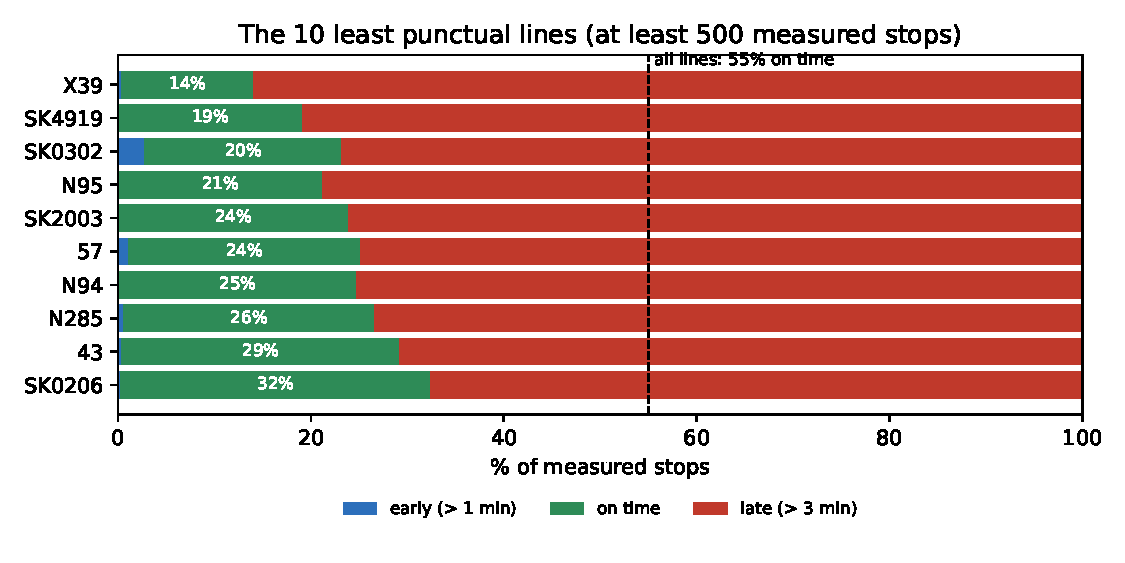
\includegraphics[width=\linewidth]{2_worst_lines.pdf}
\caption{The ten least punctual lines (at least 500 measured stops).}
\label{fig:lines}
\end{figure}


\section{Reflection}
\label{sec:reflection}
\textbf{What worked.} We measured before deciding, and several first guesses were wrong
(15-minute polling, 200 partitions, three Bronze days). Planning for reruns early made
backfills easy, and flagging problems instead of deleting rows let us change the delay limits
later without touching Bronze.

\textbf{What did not work at first.} Cron and GitHub Actions together fetched every snapshot
twice, the first Silver run on prod ran out of memory, the first volume got stuck, and the line
names skipped Bronze. All are fixed and logged in \code{docs/decisions.md}.

\begin{table}[htb]
\caption{Data we miss. Each row is counted in the Bronze metadata or the Silver quality table.}
\label{tab:missing}
\centering\footnotesize
\renewcommand{\arraystretch}{1.25}
\begin{tabularx}{\linewidth}{@{}>{\raggedright}p{2.5cm}>{\raggedright}p{1.6cm}>{\raggedright\arraybackslash}X@{}}
\toprule
What is missing & How much & Why we accept it \\
\midrule
Failed Bronze run (DNS, 29 Oct) & 1 of 7{,}778 & A trip is in many snapshots, so almost nothing is lost \\
Stops with only a predicted time & 0.2--1.8\% a day & Changes the on-time share by 0.05 points \\
Delay outliers & below 0.1\% a day & Feed errors; flagged and left out of punctuality only \\
Trips that are not in the feed & unknown & Would need the GTFS timetable \\
\bottomrule
\end{tabularx}
\end{table}

\textbf{Limitations.} One VM collects the data, so if it is down those snapshots are lost for
good. All our data is from winter time, so the read window is not tested in summer time.

\textbf{What we learned.} With a live source, collection matters most: Silver and Gold can be
rerun, a missed snapshot cannot. Our slow part was Python, not Spark, and reading less data
helped where Spark settings could not. The presentation feedback found a weak spot we had
stopped seeing ourselves. Next we would save parsed Bronze files once, add GTFS, and build a
small dashboard on Gold.


\bibliographystyle{ACM-Reference-Format}
\bibliography{references}

\end{document}
